% vim: set textwidth=78 autoindent:

%\subsection{Coordinate Capture Plugin}
\subsection{Extension Saisie de Coordonnées}

% when the revision of a section has been finalized, 
% comment out the following line:
% \updatedisclaimer

%The coordinate capture plugin is easy to use and provides the 
%ability to display coordinates on the map canvas for two 
%selected Coordinate Reference Systems (CRS).

L'extension Saisie de Coordonnées est simple d'utilisation et offre la
possibilité d'afficher des coordonnées sur la carte en sélectionnant deux
Systèmes de Coordonnées de Référence (SCR) différents.

%\begin{figure}[ht]
%   \begin{center}
%   \caption{Coordinate Cature Plugin \nixcaption}\label{fig:coordinate_capture_dialog}\smallskip
%   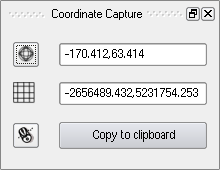
\includegraphics[clip=true, width=9cm]{coordinate_capture_dialog}
%\end{center}  
%\end{figure}

\begin{figure}[ht]
   \begin{center}
   \caption{L'extension Saisie de Coordonnées \nixcaption}\label{fig:coordinate_capture_dialog}\smallskip
   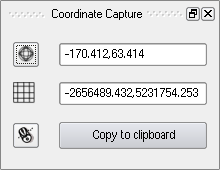
\includegraphics[clip=true, width=9cm]{coordinate_capture_dialog}
\end{center}  
\end{figure}

%\begin{enumerate}
%  \item Start QGIS, select \dropmenuopttwo{mActionOptions}{Project Properties} from 
%  the \mainmenuopt{Settings} (KDE, Windows) or \mainmenuopt{File} (Gnome, OSX) menu 
%  and click on the \tab{Projection} tab. As an alternative you 
%  you can also click on the \toolbtntwo{mIconProjectionEnabled}{projector} icon in the lower 
%  right-hand corner of the statusbar.
%  \item Click on the \checkbox{Enable on the fly projection} checkbox and select a projected 
%  coordinate system of your choice (see also Section \ref{label_projections}).
%  \item Load the coordinate capture plugin in the Plugin Manager (see Section 
%  \ref{sec:load_core_plugin}) and ensure that the dialog is visible by going to \mainmenuopt{View}
%   > \dropmenuopt{Panels} and ensuring that \checkbox{Coordinate Capture} is enabled. 
%   The cordinate capture dialog appears as shown in Figure \ref{fig:coordinate_capture_dialog}.
%  \item Click on the \toolbtntwo{geographic}{Click to the select the CRS to use for coordinate display} 
%  icon and select a different CRS from the one you selected above.
%  \item To start capturing coordinates, click on \button{Start capture}. You can now click anywhere 
%  on the map canvas and the plugin will show the coordinates for both of your selected CRS.
%  \item To enable mouse coordinate tracking click the \toolbtntwo{tracking}{mouse tracking} icon.
%  \item You can also copy selected coordinates to the clipboard.
%\end{enumerate}

\begin{enumerate}
  \item Démarrez QGIS, sélectionnez \dropmenuopttwo{mActionOptions}{Propriétés du  Projet} dans le menu 
  \mainmenuopt{Préférences} (KDE, Windows) ou \mainmenuopt{Fichier} (Gnome, OSX) 
  et appuyez sur l'onglet \tab{Système de coordonnées de référence (SCR)}.
  Vous pouvez également appuyer sur l'icône \toolbtntwo{mIconProjectionEnabled}{Statut de la projection}
  située dans l'angle inférieur droit de la barre de statut.
  \item Cochez l'option \checkbox{Autoriser la projection 'à la volée'} et
  sélectionnez le système de coordonnées de votre choix (voir également
  la Section \ref{label_projections}).
  \item Chargez l'extension Saisie de Coordonnées depuis le Gestionnaire
  d'Extension (voir la Section \ref{sec:load_core_plugin}) puis assurez-vous
  que l'extension est activée en allant dans \mainmenuopt{Vue} > \dropmenuopt{Panneaux} 
  pour vérifier que la fonction \checkbox{Saisie de Coordonnées} est cochée. 
   La fenêtre Saisie de Coordonnées apparaît alors comme indiqué dans 
  la Figure \ref{fig:coordinate_capture_dialog}.
  \item Appuyez sur l'icône \toolbtntwo{geographic}{Cliquez pour sélectionner le SCR à utiliser pour l'affichage des coordonnées} 
  et sélectionnez un SCR différent de celui que vous avez choisi plus haut.
  \item Pour lancer la capture de coordonnées, appuyez sur \button{Debuter la capture}. Vous pouvez maintenant cliquer n'importe où sur la carte et l'extension affichera les coordonnées dans chacun des deux SCR sélectionnés.
  \item Pour activer le suivi des coordonnées par le curseur appuyez sur l'icône \toolbtntwo{tracking}{Suivi du curseur}.
  \item Vous pouvez également copier les coordonnés dans le presse-papiers.
\end{enumerate}

\newpage

